% gc-termtest-C.tex

\documentclass[11pt]{article}
\usepackage{alltt}
\usepackage{enumerate}
\usepackage{syllogism} 
\usepackage{october}
\usepackage[table]{xcolor}
\pagestyle{empty}

\newcounter{aufg}
\setcounter{aufg}{0}
\newcommand{\aufgabe}[1]{\refstepcounter{aufg}\textbf{(\arabic{aufg})}[#1 points]}

\begin{document}

\textbf{Term Test C version 1}

Note that for $f(x)=\tan{}x$ the derivative is $f'(x)=\sec^{2}x$.

\aufgabe{5} The formula to work out the total resistance $R_{T}$ given two resistors $R_{1}$ and $R_{2}$ in parallel as in the diagram is
\begin{equation}
\label{eq:tiexueri}
\frac{1}{R_{T}}=\frac{1}{R_{1}}+\frac{1}{R_{2}}\notag
\end{equation}
\begin{figure}[ht]
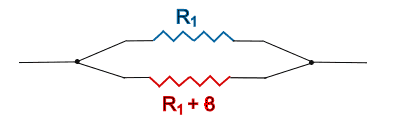
\includegraphics[scale=.7]{./resist.png}
\end{figure}
The total resistance has been measured at 3 ohms, and one of the resistors is known to be 8 ohms more than the other. Ohm is the unit for resistance, and only a positive number of ohms makes sense. Calculate $R_{1}$.

\aufgabe{5} Solution X is a 27% salt solution and Solution Y is a 20% salt solution. How much of each is needed to make 42 gallons of a 25% salt solution?

\aufgabe{5} You have 20 gallons of a 45 percent antifreeze solution. How many gallons of a 57 percent antifreeze solution needs to be added to make a 51 percent antifreeze solution?

\aufgabe{5} Solve the equation.

\begin{equation}
\label{eq:ulugheec}
\frac{3+x}{2}-\frac{2x-7}{3}=3\notag
\end{equation}

\end{document}
